\documentclass[UTF8, xcolor=table]{beamer}
\usepackage[BoldFont,SlantFont]{xeCJK}
\setCJKmainfont[BoldFont={Adobe Heiti Std},ItalicFont={Adobe Kaiti Std}]{AdobeSongStd-Light}
% \setCJKmainfont[BoldFont={Adobe Heiti Std},ItalicFont={Adobe Kaiti Std}]{SimSum} %Windows先编译使用这个字体

\usepackage{latexsym,amssymb,amsmath,amsbsy,amsopn,amstext,xcolor,multicol}
\usepackage{graphicx,wrapfig,fancybox}
\usepackage{pgf,pgfarrows,pgfnodes,pgfautomata,pgfheaps,pgfshade}
\usepackage{thubeamer}
\usepackage[backend=bibtex,sorting=none]{biblatex} % [参考文献格式](https://www.sharelatex.com/blog/2013/07/31/getting-started-with-biblatex.html) %mac IEEE not found
\usepackage{array}
\usepackage{bm}
\usepackage{caption}
\RequirePackage[font=footnotesize]{subcaption}
\usepackage{multirow}
\usepackage{booktabs}
\usepackage{tikz}
\usepackage{tikzscale}
\usepackage{animate}

\defbibheading{bibliography}[\bibname]{} %avoid printbibliography 自动生成目录
\addbibresource{../main.bib}
\setbeamertemplate{bibliography item}[text] 

\usepackage{boxedminipage} %for: bvh border
\def\fourgraphicswidth{0.35} %0.3\textwidth

\usepackage{algorithm} %%format of the algorithm
\usepackage{algpseudocode}
\floatname{algorithm}{算法}
\renewcommand{\algorithmicrequire}{\textbf{输入:}} % Use Input in the format of Algorithm
\renewcommand{\algorithmicensure}{\textbf{输出:}} % UseOutput in the format of Algorithm
\algrenewcommand{\algorithmiccomment}[1]{ $//$ #1}

\usepackage{listings}
\renewcommand\lstlistingname{代码}
\renewcommand\lstlistlistingname{代码}

\lstset{framexleftmargin=1.4em,
        xleftmargin=1.8em,
        basicstyle=\ttfamily\small,
        %frame=shadowbox, numberstyle=\tiny, breaklines=true,
        frame=single,
        numberstyle=\tiny, breaklines=true,
        keywordstyle=\color{blue!70}\bfseries,
        %commentstyle=\color{red!50!green!50!blue!50},
        rulesepcolor=\color{red!20!green!20!blue!20},
        numbers=none,fontadjust=true}
\lstdefinelanguage{shader}{morekeywords={uniform, layout, uniform, vec2, vec3, vec4, in, out, gl_Position, dot, flat, int ,float, gl_VertexID, xyz, w, x, y, z, location, version, sampler2DRect, bgr, gl_FragData, texture2DRect, gl_TexCoord,for,xy},morecomment=[l]{//}}

\begin{document}

\setbeamerfont{footnote}{size=\tiny}
\setbeamerfont{caption}{size=\scriptsize}
\setbeamertemplate{caption}[numbered]
\setbeamerfont{subsection in toc}{size=\footnotesize}
\renewcommand*{\bibfont}{\footnotesize}

\graphicspath{{../}}

\title[融合长短记忆神经网络与卷积特征学习的图像语义分割]{中山大学本科毕业论文演示文稿非正式模版}
\author[陈冠英]{}%{(申请中山大学工学学士学位论文答辩报告)\\ \vskip 20pt 学~~~~~~生:陈~冠~英}
\institute[中山大学~电子信息与工程学院~\&~自动化]{}%{\small \vskip 38pt 电子信息与工程学院~自动化}
\date{} %{\small \vskip -17pt二〇一六年五月}

%% make title %%
\frame{
	\titlepage
	\vspace{-23mm}
	\begin{figure}[h]
		\centering
		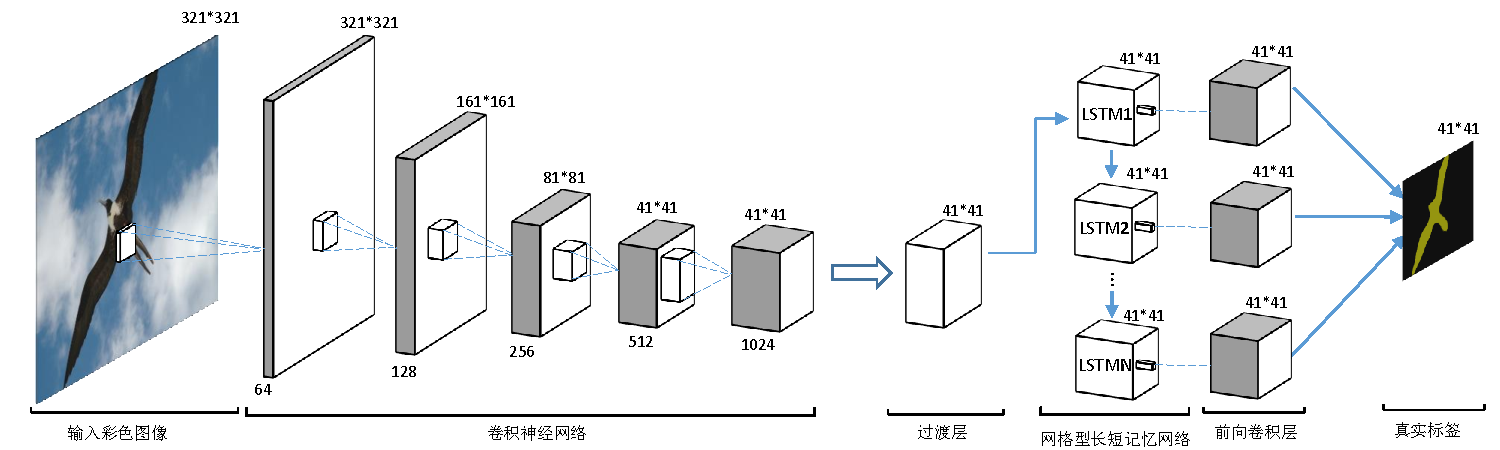
\includegraphics[width=\textwidth]{image/illustration/networkstructure.pdf}
	\end{figure}
}

\frame {
	\frametitle{目录}
	%\begin{multicols}{2}
	\tableofcontents[sections={<1-7>}]
}

%%
% 引言或背景
% 引言是论文正文的开端,应包括毕业论文选题的背景、目的和意义;对国内外研究现状和相关领域中已有的研究成果的简要评述;介绍本项研究工作研究设想、研究方法或实验设计、理论依据或实验基础;涉及范围和预期结果等。要求言简意赅,注意不要与摘要雷同或成为摘要的注解。
% modifier: 黄俊杰(huangjj27, 349373001dc@gmail.com)
% update date: 2017-04-15
%%

\chapter{引言}
\label{cha:introduction}
\section{选题背景与意义}
\label{sec:background}
让机器节省甚至替代人力一直是科技发展的大方向。自动驾驶汽车,一种通过传感器和电脑实现无人驾驶的智能汽车,则是近些年来越来越受到关注的一个研究热点。如果自动驾驶技术能在生活中得到广泛应用,那么人们的生活质量将大幅提高。举两个很贴近校园生活的例子:很多学校都有校内接送学生的电动车,它的时间和线路相对固定,驾驶巴士的司机常年做着重复劳动,十分枯燥;很多同学喜欢叫外卖,因此无数的递送员每天奔波于商家和宿舍之间,还经常因为无法按时送达被投诉。但假如能应用成熟的自动驾驶技术,这样的情况将得到极大改善。不仅如此,在国家快速现代化发展的大环境下,自动驾驶还可以缓解城市交通拥堵、交通事故发生频繁等问题。所以,自动驾驶技术的发展对于国家和社会具有重要意义。

虽然自动驾驶技术距离广泛应用还有一定的距离,但相关研究工作已经在国内外各大企业和高校如火如荼地展开。为了方便区分和定义自动驾驶的程度,国际自动机工程师学会(SAE)提出了一套分级标准,将自动驾驶分为了L0到L5六个等级(如图1-1)。其中L0和L1实现自动化的程度非常低,需要人类驾驶员执行几乎所有操作。而到了L2,控制方向和加减速的操作就可以由汽车自己完成,驾驶员需要监视,准备随时接管以完成其他操作。到了L3,驾驶员已经可以解放手脚了,但仍需保持注意力集中。而L4和L5则已经无需驾驶员的控制,完全由汽车自己掌握全部操作,只是L4对道路环境有特殊要求。目前很多汽车制造商的技术都达到了L2级别,比如Tesla的Autopilot 2.0和Volvo的S60。谷歌测试中的无人车处在L3的阶段。而硅谷一家2016年成立的公司Nuro声称他们的配送车可以不用人类驾驶员,也就是至少达到了L4的水平。
\begin{figure}[h]
	\centering
	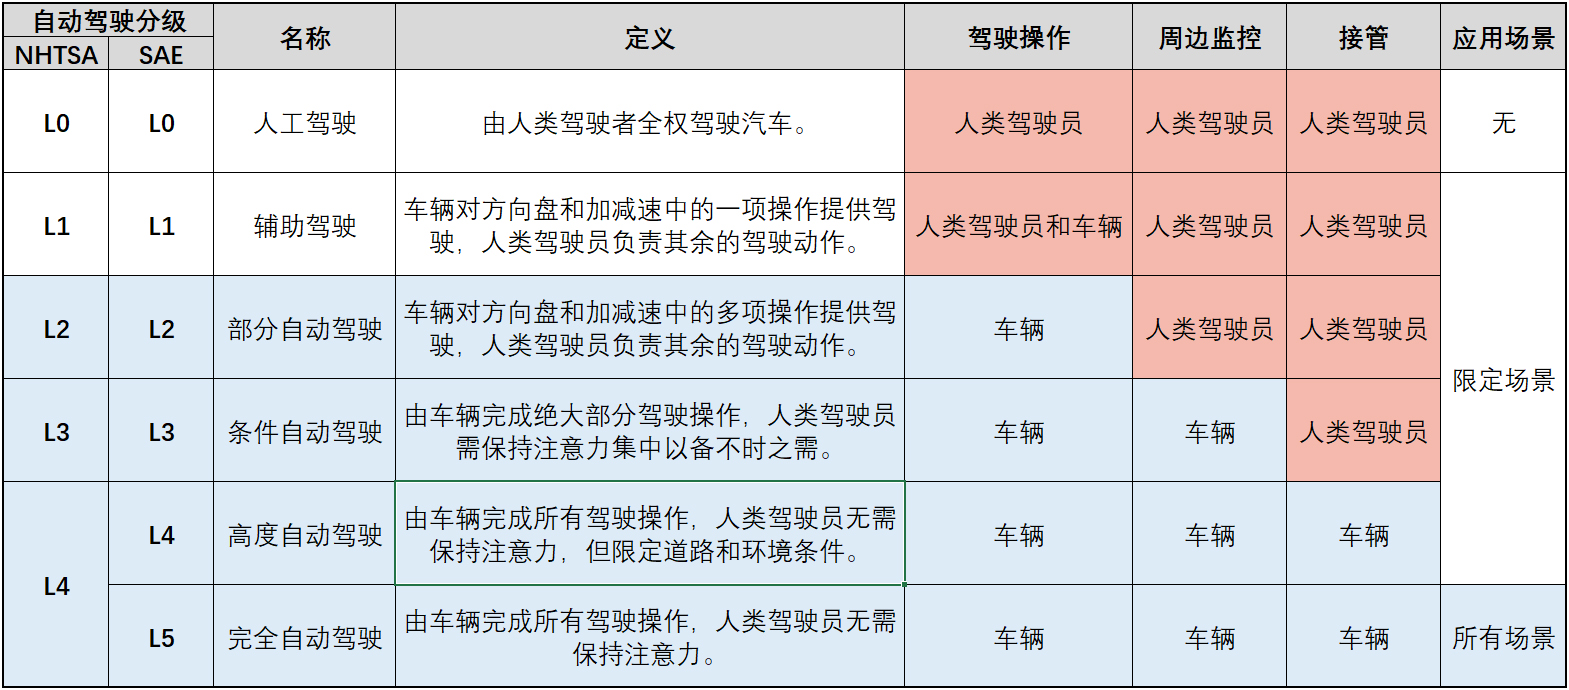
\includegraphics[width=0.5\textwidth]{image/自动驾驶等级.jpg}
	\caption{SAE提出的自动驾驶等级}
 	\label{fig:1-1}
\end{figure}


自动驾驶中的一大难点是环境感知,即采用什么样的传感器,以及如何将传感器采集的环境数据转化为机器可以理解的数据。对于这个问题,不同的实验室有不同的解决方案。Tesla使用的是视觉摄像头。由于视觉摄像头成本低廉,且图像检测算法已经较为成熟,所以纯视觉方法应用更为广泛。但是视觉摄像头,无论单目还是多目,都很难捕捉到准确的三维信息,因为它们很容易受到环境中光线变化、障碍物遮挡等的影响。谷歌旗下的Waymo和百度的Apollo则更多使用激光雷达。激光雷达的优点在于稳定性高,对空间感知能力强。然而它的成本高昂,且基于它采集的三维数据的算法复杂度较高,所以如何将其很好地应用还有待进一步研究。

\section{问题描述}
\label{sec:problem_description}
自动驾驶场景下的三维物体追踪,主要目标是:基于激光雷达在实际道路场景采集的三维点云数据(kitti数据集),追踪其中的多辆汽车,用三维的立方体框将它们在点云中准确地标识出来。由于数据集由一段一段连续的点云流构成,帧与帧之间不存在剧烈的变化,所以相邻帧之间的特征图具有一定的共性。如果我们能对点云流的这一特点加以利用,则将进一步提升最终的效果。

\section{本文的工作}
\label{sec:key_work}
针对上文提到的主要目标和优化方向,本项目融合了两种开源框架。其中,Voxelnet中的特征学习(feature learning)是框架的主要部分,而Detect to Track(下文简称D&T)中的相关层(correlation layer)则可以很好地发掘相邻帧之间特征的相似性。为了适配相关层的输入和输出,我们对点云读取方式和损失函数计算方式也做出了相应的调整。总结本文具体的创新和贡献如下:
\begin{itemize}
	\item 采用合并相邻两帧的方式读取点云数据。
	\item 采用Voxelnet学习特征,同时用D&T的相关层发掘相邻帧的相似性。
	\item 在损失函数中加入相关损失(correlation loss)。
\end{itemize}

\section{论文结构与章节安排}
\label{sec:arrangement}
本文共分为五章,各章节内容安排如下:

第一章引言。

第二章综述。

第三章方法、原理和框架。

第四章实验和结果。

第五章总结与展望。


\chapter{综述}
\label{cha:review}
本章综述,将对整个项目基于的数据集和采用的方法做一个简要概述。首先是激光雷达以及国外研究团队用它采集到的kitti数据集:整个框架的训练、验证和测试都在该数据集上完成。由于本项目只采用了激光雷达采用的三维点云数据集,所以纯RGB图像方法或者图像和点云结合的方法将不被提到。接下来是分别对点云物体检测和视频流物体追踪两个领域主要方法的介绍。本项目融合的Voxelnet和D&T就分别来自这两个领域。

\section{激光雷达}
\label{LiDAR}

\section{kitti数据集}
\label{sec:kitti}

\section{点云物体检测}
\label{sec:Detection_in_Point_Cloud}

\section{视频流物体追踪}
\label{sec:Tracking_in_Video}




\chapter{研究方法}
\label{cha:method}

%% chapter 4 dataset, network structure, experiment and result
\chapter{实验与结果}
\label{cha:experiment}


%%
% 结论
% 结论是毕业论文的总结,是整篇论文的归宿,应精炼、准确、完整。结论应着重阐述自己的创造性成果及其在本研究领域中的意义、作用,还可进一步提出需要讨论的问题和建议。
% modifyer: 黄俊杰(huangjj27, 349373001dc@gmail.com)
% update date: 2017-04-13
%%

\chapter{总结与展望}
\section{工作总结}
\indent 本文所述框架是基于两种效果显著的三维物体检测与追踪开源框架改进而来。
\indent 然而,在追踪取得较高精确度的同时,该框架的速度还有待提升。目前的追踪速度只有约2秒每帧,尚不能达到自动驾驶的要求。
\section{研究展望}
\indent 随着硬件设备的性能不断提高,伴随5G时代的到来,自动驾驶汽车的各个部件之间的通讯将更加稳定高效,而日渐成熟的三维物体检测与追踪技术也将为人们带来更安全和舒适的自动驾驶体验。
\section{致谢}
\subsection*{致谢}
\frame{
	\frametitle{致谢}
	\begin{block}{感谢每一个帮助过我的人}
	\begin{itemize}
		\item 首先要感谢的是我的指导老师的悉心指导
		\item 感谢师兄师姐、同学的帮助
		\item 感谢家人的支持
		\item 感谢答辩委员会的聆听和指导
	\end{itemize}
	\end{block}
	\vspace{-1em}
	\note{
		我的展示到此结束,我要感谢我的指导老师,师兄师姐同学,家人还有答辩委员会老师的聆听与指导。谢谢大家
	}
}
\frame{
	\frametitle{Q \& A}
	\begin{block}{Questions?}
	 ~\\ ~\\
	 \center{\Large{Thank you!}}
	 \\ ~\\ ~\\ ~\\ ~\\ 
	\end{block}
	\note{
		现在是问答时间。请问老师们对我的展示有什么疑问?
	}
}



\end{document}
